% Pursuing Stacks (cotes 134-2 to 134-8): archive cote 134-6, site page 32 (PDF page 33), typescript page 350.
% typescript. Draft compared: ps5.tex:2901-2973.
% AI-transcribed by Claude Opus 5.5 (claude-opus-5-5, adaptive thinking, effort high), Message Batches API, batch ps3 (msgbatch_01XdFmuVVBAcgc7EFxdtCqsj), 2026-11-12; reviewed against both supplied scan halves; see CHECK_DECISIONS.tsv.
\scanpage{134-6/32}
\mspage{350}

\xout{We now can prove the foll}
The preceding reflections thus prove the following afterthought to
theorem 1 of section 79 :

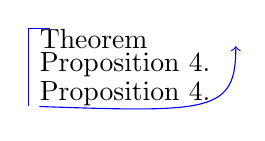
\begin{tikzpicture}[baseline=(ph.base)]\node[inner sep=0pt] (ph) {\deleted{\uline{Proposition} 4.}};\node[anchor=south west,inner sep=0pt] (pt) at ([yshift=.3ex]ph.north west) {\deleted{\hand{\unsure{Theorem}}}};\node[anchor=north west,inner sep=0pt] (pb) at ([yshift=-.3ex]ph.south west) {\hand{Proposition 4.}};\draw[color=blue] ([xshift=-.4em]pb.south west)--([xshift=-.4em]pt.north west)--([xshift=.4em]pt.north west);\draw[color=blue,->] (pb.south west) .. controls ([yshift=-.5ex]pb.south east) and ([xshift=.9em,yshift=-.5ex]pb.south east) .. ([xshift=.9em,yshift=.5ex]ph.north east);\end{tikzpicture} Let $(M,M_c)$ be a contractibility structure, $A$ a small
category, $i\colon A\hand{\longrightarrow} M$ a functor factoring through $M_c$ . \xout{We assume} Let
moreover $\underline{W}$ be a basic localizer satisfying L\tikz[baseline=(lo.base)]{\node[inner sep=0pt] (lo) {o};\draw ([xshift=-.4ex,yshift=.7ex]lo.north) .. controls ([yshift=-.1ex]lo.north) .. ([xshift=.4ex,yshift=.7ex]lo.north);\draw ([xshift=-.4ex,yshift=-.8ex]lo.south) .. controls ([yshift=.2ex]lo.south) .. ([xshift=.4ex,yshift=-.8ex]lo.south);}c 4) . We assume $A$
\xout{totally W} \uline{strictly totally $\underline{W}$-aspheric}, i.e. totally $\underline{W}$-aspheric and
moreover any object of $A$ has a section (over $e_{A^\wedge}$) .

a) The homotopy structure $h_{\underline{W}_A}$ on $A^\wedge$ is equal to the canonical
homotopy structure $h_{A^\wedge}$ defined by 0-connected intervals, and equal
also to the homotopy structure $h$ defined by intervals coming from $A$ :
\[ (6) \qquad h = h_{\underline{W}_A} = h_{A^\wedge} \ . \]
In what follows, we assume $A^\wedge$ endowed with this homotopy structure,
and denote by $A^\wedge_c$ the set of all contractible objects in $A^\wedge$. We equal-%
ly endow $A^\wedge$ with it's canonical $\underline{W}$-asphericity structure , and $M$ with
the $\underline{W}$-asphericity structure associated to it's contractibility struc-%
ture $M_c$ . With these conventions:

b) T\over[typed]{h}{h}e following conditions on $i$ are equivalent, where
\[ i^* : M \hand{\longrightarrow} A^\wedge \]
is the functor defined as usual in terms of $i$:

(i) $i^*$ is compatible with the homotopy structures (cf. criteria on
pages 251-252), which can be expressed also by
\[ i^*(M_c) \hand{\subset} A^\wedge_c \]
(a condition undependent from $\underline{W}$\hand{,} in view of a)).

(ii) $i$ is $\underline{W}$-aspheric , i.e.
\[ \xout{\illegible{1}}M_{\underline{W}} \over{\illegible{1}}{\subset}\hand{(i^*)^{-1}}\hand{(}A^\wedge_{\underline{W}}) \ , \]
(where $M_{\underline{W}}$ and $A^\wedge_{\underline{W}}$ are the sets of \inserted{$\underline{W}$-} aspheric objects in $M$ and \inserted[typed]{in $A^\wedge$).}

(iii) (F\over[typed]{o}{o}r a given full subcategory \inserted{$C$} of $M$ generating the contracti-%
bility structure $M_c$):
\[ i^*(C) \hand{\subset} A^\wedge_{\underline{W}_o} = \text{set of 0-connected objects of } \inserted[typed]{A^\wedge.} \]

c) Assume these conditions hold, and moreover that the contrac-%
tibility structure \xout{$\unsure{M_c}$}\hand{of} $M$ is non trivial. T\over[typed]{h}{h}en $A$ is a strict $\underline{W}$-test
category.

\margin{32}

% Visual collation: both supplied image halves inspected; see CHECK_DECISIONS_134_7_8.tsv.
